%% References--------------------%-------------------------------
\renewcommand{\bibname}{References}%Set the name of the bibliography here
\bibliographystyle{src/elsarticle-aps}
\cleardoublepage
\phantomsection %Ordering here is important; place this line before calling \bibliography{}...
\bibliography{src/bib_link}
\addcontentsline{toc}{chapter}{\texorpdfstring{\uppercase{\bibname}}{\bibname}}%...and place this line after calling \bibliography{}
\vspace*{\stretch{1}}
\renewcommand{\arraystretch}{1.3} % set tabular line spacing
\begin{table*}[hb]
\begin{center}
\subsubsection*{Colophon}
\begin{tabular}{p{0.45\columnwidth}|p{0.45\columnwidth}} 
\raggedleft Font&Adobe Utopia 10\,pt with \texttt{mathdesign~v1.55}\\
\raggedleft \TeX{} Implementation&Mik\TeX{} 2.9\\
\raggedleft IDE/Text Editor&\TeX nicCenter 1.0 RC 1\\
\raggedleft Computer Hardware&HP Pavilion dv6226us Notebook PC\\
\raggedleft Operating System&Windows 7 Home Premium 32-bit\\
\multicolumn{2}{c}{}\\
\raggedleft Cloud-based LaTeX editor&Overleaf\\
\raggedleft Version control&GitHub\\
\end{tabular}
%\caption[Time of document compilation]{This is a table showing when this document was made.}
\label{colo}
%\caption[Colophon]{Colophon}
\end{center}
\end{table*}

\twoappendix
%\input{More_Files/Field_Map_Data} %full field map
\cleardoublepage
%\thispagestyle{plain}
%\setcounter{secnumdepth}{-1} 
%\chapter[\texorpdfstring{APPENDIX}{Appendix}]{Field Map}
\chapter{Field Map}
%\addcontentsline{toc}{chapter}{\texorpdfstring{APPENDIX}{Appendix}}
\label{field_map_data}
\renewcommand{\arraystretch}{0.8} % set array line spacing
\renewcommand{\tabcolsep}{1.9mm} % set array column separation
\begin{table}[ht]
\centering
\begin{tabular}{r|d{1}d{1}d{1}d{1}d{1}d{1}d{1}d{1}d{1}d{1}}
\hline
\multicolumn{1}{c|}{\multirow{2}{*}{$z$}} &\multicolumn{10}{c}{$\rho$}\\ %\cline{2-11}

\input{Axial-field.txt}
\hline
\end{tabular}
\caption{Average axial field strength $\mathscr{B}_z$ of the HELIOS solenoid in gauss. }
\label{axial_field}
\end{table}

\begin{table}[t]
\centering
\begin{tabular}{r|d{1}d{1}d{1}d{1}d{1}d{1}d{1}d{1}d{1}d{1}}
\hline
\multicolumn{1}{c|}{\multirow{2}{*}{$z$}} &\multicolumn{10}{c}{$\rho$}\\ %\cline{2-11}
\input{Radial-Field.txt}
\hline
\end{tabular}
\caption{Average radial field strength $\mathscr{B}_\rho$ of the HELIOS solenoid in gauss.}
\label{radial_field}
\end{table}

The field values presented in this appendix represent the interpolated field map matrix used in the simulations.  It is based on the 21,240 point field map discussed in Chapt.~\ref{solenoid}.  For each combination of ($z$,$\rho$) in the original field map, the azimuthal variations in the measured field have been averaged.  The value of the magnetic field at fixed intervals of $\Delta z=5$\,cm are interpolated from the azimuthally-averaged values in a manner similar to the fit shown in Fig.~\ref{map}.

%\thispagestyle{myheadings}
%\markright{APPENDIX FIELD MAP}
 %averaged field map
%\backmatter

\chapter{Afterword}
\label{fig_notes}
The bulk of the material discussed in this dissertation was originally published by the author and collaborators in Ref.~\cite{Lighthall_2010}.  Each of the figures from this reference appear in this dissertation with the modifications listed below.
\renewcommand{\arraystretch}{1.3} % set array line spacing
\begin{table*}[ht]%
  \centering
  \begin{tabular}{lll}
    \hline
    Ref.~\cite{Lighthall_2010}&Current&Modifications\\
    \hline \hline
    Fig.~1&Fig.~\ref{schematic}&none; same file\\
    Fig.~2&Fig.~\ref{analytic}&panels c) and d) are added\\
    Fig.~3&Fig.~\ref{map}&$\rho=45$\,cm is added, only measured points are shown\\
    Fig.~4&Fig.~\ref{solenoid}&none; same file\\
    Fig.~5&Fig.~\ref{psd_test}&threshold cutoff is plotted\\
    Fig.~6&Fig.~\ref{psd_energy}&``counts per'' units added\\
    Fig.~7&Fig.~\ref{psd_pos}&ROOT histograms are used in place of grace plots\\
    Fig.~8&Fig.~\ref{pcb}&none; same file\\
    Fig.~9&Fig.~\ref{array_pic}&none; same file\\
    Fig.~10&Fig.~\ref{sim_plots}&none; same file\\
    Fig.~11&Fig.~\ref{hTOF}&``counts per'' units added\\
    Fig.~12&Fig.~\ref{cezg_350}&none; same file\\
    Fig.~13&Fig.~\ref{hEZ}&acceptance cutoff is labeled\\
    Fig.~14&Fig.~\ref{double}&acceptance cutoffs are plotted\\
    Fig.~15&Fig.~\ref{qval}&$x$-scale expanded, states labeled\\
    Fig.~16&Fig.~\ref{angdist2}&figure in two panels, data from Ref.~\cite{Mermaz_1971} plotted\\
    \hline
  \end{tabular}
  \caption[Comparison of reproduced figures.]{Comparison of reproduced figures.  Each of the 16 figures in Ref.~\cite{Lighthall_2010} appear in some form in this document.}
  \label{fig_corr}
\end{table*}
%\singlespace
%\pangram{80}
%\noindent\rule{\textwidth}{1pt}\newpage
%\doublespace
%\pangram{40}
%\noindent4rule{\textwidth}{1pt}\newpage
%\begin{spacing}{2}
%\pangram{40}
%\end{spac4ng}
%\noindent\rule{\textwidth}{1pt}\newpage
\chapter{Corrigenda \& Addenda}
\label{changes}
\begin{spacing}{1.55}
%\singlespace
\newcommand{\code}[1]{{\color{note_gray}#1}}
Table~\ref{history_table} shows the revision history of this document prior to publication by UMI \cite{Lighthall_2011}.  Given below is an exhaustive list of changes made to this document since June 2011 after being accepted by the Western Michigan University Graduate College.  Section~\ref{toclass} summarizes the changes related to adoption and development of the thesis template document class \texttt{wmu-thesis.cls}. Section~\ref{errors} lists any corrections, e.g., of typographical errors, 
made to the text.  
\begin{table}[ht]%
 \mmddyydate % set date format
\renewcommand{\arraystretch}{1.3} % set array line spacing
\centering
\begin{tabular}{ccllll}
% Revision History ------------%-------------------------------
\hline
Draft&Format&Date&Submitted to&Chapters&Comments\\ \hline \hline
0 &.tex&  \formatdate{15}{02}{09} &---&---&created\\
1 &.pdf&  \formatdate{24}{08}{10} & AHW& all\\
2 &.pdf&  \formatdate{19}{11}{10} & AHW& 7\\
3 &.pdf&  \formatdate{14}{12}{10} & AHW& 5,7\\ 
4 &.pdf&  \formatdate{02}{02}{10} & AHW& 5,7 \\
5 &.pdf&  \formatdate{20}{02}{10} & AHW& 9 \\
6 &.pdf&  \formatdate{14}{03}{10} & AHW& 14\\
7 &.pdf&  \formatdate{22}{03}{10} & AHW& 10\\
8 &.pdf&  \formatdate{30}{03}{10} & AHW& 12\\
9 &.pdf&  \formatdate{03}{04}{10} & AHW& 11\\
10 &.pdf&  \formatdate{05}{04}{10} & AHW& 16\\
11 &.pdf&  \formatdate{22}{04}{10} & AHW& all\\
12 &.pdf&  \formatdate{24}{04}{10} & AHW& 10,12,14\\
13 &.pdf&  \formatdate{28}{04}{10} & AHW, BBB, DH, KK &all\\
14 &.pdf&  \formatdate{30}{04}{10} & AHW, BBB, DH, KK& all&approved\\
15 &.pdf&  \formatdate{27}{05}{10} & JWH&all\\
16 &.pdf&  \formatdate{15}{06}{10} & JWH &all&accepted\\ \hline
\end{tabular}
\caption[Revision history pre-publication.]{Revision history pre-publication.  The file format and completion date of each revision is given.  The content of each draft is listed including who the draft was sumbitted to.}
\label{history_table}
\end{table}

%Please email the author at \href{mailto:jonathan.c.lighthall@wmich.edu}{jonathan.c.lighthall@wmich.edu} to report any errors not listed there.
Section~\ref{adds} lists any new content added to the document. 
Items printed in \code{ gray} are code-level alterations affecting compiling and the resulting PDF output, but not the printed document.  In each section, changes are listed in the order they appear (with respect to the code).

\section{Dissertation Template Class File}
\label{toclass}
In the accepted version of this document, certain aspects of the layout of the front matter and back matter were not in strict accord with the \textit{Guidelines} published by the Graduate College.  Those discrepancies are corrected in this document.  The layout modifications implemented in the accepted version of this document have subsequently been incorporated in a \LaTeX{} class file.
\subsection{Layout and Formatting}
\label{class_details}
Listed below is a summary of changes to the layout and formatting of the document---as compared to the accepted version---made by the class file.  
\begin{itemize}
\setlength{\itemsep}{-4pt}	
	\item The vertical spacing on the abstract and title pages is adjusted to meet requirements based on the printed output.  See note in \S\,\ref{orig}.
	\item \code{Reference to two-column documents is removed.}
	\item \verb|\voffset| is increased by the length \verb|\tocskip| in the front matter to position the headers.  
	\item \code{In the absence of \texttt{abstract\_body.text}, instructions for the abstract are printed.}
	\item The output of the optional command \verb|\draftno| is removed from the abstract.
	\item \code{The degree abbreviation is set by a document class option, e.g. \texttt{[phd]}.}
	\item \code{If the abstract spans two pages, the second page starts at the same position as the headers in the rest of the front matter.}
	\item \code{The page number of the title page is changed to p.~i.}
	\item \code{The command \texttt{\char`\\draftno} is added to the title (on the title page only).} See note in \S\,\ref{orig}.
	\item \code{The project type and degree name are set by a document class option, e.g. \texttt{[phd]}.}
	\item \code{The copyright page is unnumbered in the PDF.}
	\item Headers of the form ``\textit{<Section>}---Continued'' are added to the front matter.  \code{ This correction requires the inclusion of  the \texttt{fancyhdr} package.}
	\item After the copyright page, the front matter is enclosed in a new environment to reduce the \verb|\textheight| by \verb|\tocskip| without affecting the vertical spacing in the rest of the document.
	\item The acknowledgments section heading is moved outside of the \texttt{singlespace} environment.  The vertical spacing of the heading is the same as other unnumbered chapters.  See note in \S\,\ref{orig}.
	\item \code{The section headings in the front matter are raised by \texttt{\char`\\tocskip}.}
		%\item \code{The \texttt{\char`\\aknoname} name declaration is moved from \texttt{ackn.tex} to \texttt{front\_matter.tex} (deprecated)}
	\item \code{In the absence of \texttt{acknowledgments\_body.text}, instructions for the acknowledgments are printed.}
	\item \code{A PDF bookmark for the Table of Contents is added.}
	\item  The running page headers produced with the \verb|\pagestyle{headings}| command have been recreated within the context of the \texttt{fancyhdr} package.  The default behavior is no headers.  See notes in sections~\ref{adapt} and \ref{orig}.
	\item Tables and figures in the appendices are removed from the List of Tables and List of Figures, respectively.  See note in \S\,\ref{orig}.
	\item The command \verb|twoappendix| is added, which produces an appendix page.
	\item The command \verb|oneappendix| is added.
			\vspace{-4pt}
			\begin{itemize}
			\setlength{\itemsep}{-2pt}
			\item The Table of Contents entry for the appendix chapter is APPENDIX.
			\item The chapter letter is removed from the (single) chapter heading.
			\item The chapter letter is removed from page headers.
		\end{itemize}
	\item Tab leaders are added to the first-level (chapter) entries in the Table of Contents.
		
\end{itemize}

\subsection{Adaptations}
\label{adapt}
Required changes made to the original files to adapt the document to the new class are summarized below.  Of the original 31 \texttt{.tex} files used to compile the document, four files are modified (changes listed below), five files are omitted, and one file is added in the adoption of the class file.  This leaves a total of 27 \texttt{.tex }files.
\begin{itemize}
	\setlength{\itemsep}{-4pt}
	\item The following changes were made to the parent (top-level) file \texttt{JC\_Lighthall\_Thesis.tex}.
		\vspace{-4pt}
		\begin{itemize}
			\setlength{\itemsep}{-2pt}
			\item The document class is changed from the \LaTeX{} standard \texttt{book.cls} class to \texttt{wmu-thesis.cls}, version~1.2.  The document class declaration is changed to
				\begin{quote}
					\begin{verbatim}
						\documentclass[phd,abstract,ackno,listtab,listfig,orig]{wmu-thesis}
					\end{verbatim}
				\end{quote}%\vspace{4pt}
		 	\item The command \verb|\VerbatimFootnotes| is omitted, as it causes footnote warnings from \verb|hyperref|.
			\item The commands within the files \texttt{front\_matter.tex}, \texttt{abst.tex}, \texttt{titl.tex}, \texttt{copy.tex}, 
			and \texttt{ackn.tex}, have been absorbed into \texttt{wmu-thesis.cls}.
			\item The instances of the command \verb|\pagestyle{headings}| are omitted, replaced with
				\begin{quote}
					\verb|\lhead{\textsl{\leftmark}}|
				\end{quote}
		\end{itemize}
	\item The body of the acknowledgments, previously found in \texttt{ackn.tex} is moved to \verb|abstract_body.tex|.
	\item Commands in \texttt{first.tex} are updated as follows.
		\vspace{-4pt}	
		\begin{itemize}
			\setlength{\itemsep}{-2pt}
			\item All instances of \verb|\newcommand| are changed to \verb|\renewcommand|.
			\item The command \verb|draftno| is removed from the argument of \verb|\thesistitle|.  The argument of the command \verb|\draftno| is preceded by \verb|\\| and followed by \verb|\vspace{-1.0\baselineskip}| to maintain vertical spacing on the title page.	(see note in \S\,\ref{class_details}). 
			\item The commands \verb|\departmentname| and \verb|\adviname| are added.
		\end{itemize}
	\item The margin and spacing commands in \texttt{layout.tex} are commented out and moved to the class file.
\end{itemize}

\subsection{Exceptions}
\label{orig}
Listed below are the default features of the class file which are suppressed in this document to maintain consistency with the accepted version.  These changes are implemented with the document class option \texttt{[orig]}.
\begin{itemize}
	\setlength{\itemsep}{-4pt}
	\item The vertical spacing on the abstract and title pages is preserved from the accepted version.  The vertical spacing is based on measurements using the ruler in Adobe Acrobat (as apposed to measuring the printed output).
	\item The acknowledgments section heading is moved back inside the \texttt{singlespace} environment.  This change is made in order to constrain the acknowledgments section to one page and thus preserve the page numbering.
	\item Running page headers are included.
	\item The tables in the appendix are listed in the List of Tables.
\end{itemize}

\section{Corrections}
%\subsection{Errata}
\label{errors}
Listed below are errors found in the accepted version of the document.  This list may be repeated at the end of the document in the form of an errata sheet to be included with the bound printed copies of the original document.  Please email the author at \href{mailto:lighthall@triumf.ca}{lighthall@triumf.ca} to report any errors not listed here.  Page numbers refer to the original text.  Repeated errors are tallied in gray.
\begin{itemize}
\setlength{\itemsep}{-4pt}	
    \item p.~i, l.~16---The penultimate line on the title page should read ``Kalamazoo, Michigan''
  \item p.~iii, ll.~3--4---The \listtablename{} is on page viii and the \listfigurename{} is on page ix.
  \item p.~x, l.~7---In the entry for Fig.~6.2, the repeated ``at'' should be deleted. \code{(1)}
  \item p.~6, l.~13---A hyphen is missing in ``half lives''
  \item p.~11, l.~17---The expression ``\ldots energy transfered\ldots'' should read ``\ldots energy transferred\ldots'' \code{(1)}
  \item p.~12, l.~3---The expression``\ldots my be written\ldots'' should read ``\ldots may be written\ldots ''
  \item p.~14, l.~13---The expression ``\ldots transfered to\ldots'' should read ``\ldots transferred to\ldots'' \code{(2)}
  \item p.~17, l.~10---The expression``\ldots do no have\ldots'' should read ``\ldots do not have\ldots ''
  \item p.~16, Fig.~2.4---The expression ``Shown here\ldots'' should read ``Shown here are\ldots'' 
  \item p.~20, l.~16---The abbreviation ``Chap.'' should read ``Chapt.'' \code{(1)}
  \item p.~23, l.~19---The expression ``\ldots transfered in\ldots'' should read ``\ldots transferred in\ldots''	\code{(3)}
  \item p.~24, l.~10---The expression ``will loose'' should read ``will lose''
  \item p.~30, ll.~1,4---The abbreviation ``Chap.'' should read ``Chapt.'' \code{(2,3)}
  \item p.~34, l.~15---A space should be added after ``\ldots unknown spins.'' 
  \item p.~35, l.~5---A space should be added after ``\ldots to produce the secondary radioactive beam.'' 
  \item p.~39, l.~14---The repeated should be ``at'' should be deleted. \code{(2)}
  \item p.~41, l.~19---The expression``colinearly'' should be changed to ``collinearly''
  \item p.~44, l.~13---The repeated ``as'' should be deleted.
  \item p.~47, l.~2---A space should be added in ``separatedby''
  \item p.~47, l.~6---The expression ``Eq~3.12'' should read ``Eq.~3.12''
  \item p.~57, l.~10---A space should be added in ``defined;therefore''
  \item p.~59, l.~12---``kEV'' should be changed to ``keV''
  \item p.~62, l.~9---A space should be added in ``unperturbed.The''
  \item p.~63, l.~11---The expression ``\ldots an 20\,cm\ldots'' should read ``\ldots a 20\,cm\ldots''
  \item p.~64, l.~2---The abbreviation ``Chap.'' should read ``Chapt.'' \code{(4)}
  \item p.~71, l.~10---A space should be added in ``sample,the''
  \item p.~73, l.~26---The expression ``acutal'' should read ``actual''
  \item p.~78, l.~7---A space should be added in ``position.The''
  \item p.~78, l.~8---The repeated ``and'' should be deleted.
  \item p.~78, l.~17---The expression ``to asses the'' should read ``to assess the'' \code{(1)}
  \item p.~84, l.~3---The expression ``to asses the'' should read ``to assess the'' \code{(2)}
	\item p.~86, l.~17---The expression ``\ldots withan average gap\ldots'' should read ``\ldots with an average gap\ldots''
	\item p.~90, l.~10---The expression ``\ldots as apposed to\ldots'' should read ``\ldots as opposed to\ldots''
	\item p.~94, l.~21---The repeated ``is'' should be deleted
	\item p.~96, l.~15---The energy of the $\alpha$-particle emitted in the decay of $^{148}$Gd is 3.18\,MeV.%, not 3.27\,MeV, which is the $Q$-value of the decay. 
	\item p.~101, l.~10---The expression ``\ldots shows such a for\ldots'' should read ``\ldots shows such a fit for\ldots''
	\item p.~104---In Fig.~9.8, the $x$-axis of the plots should be labeled ``X (relative position)''
	\item p.~106---The second term under the square root on the second line of Eq.~10.1 is squared.
	\item p.~112, l.~4---The abbreviation ``pg.'' should read ``p.'' \code{(1)}
	\item p.~114, l.~20---The expression ``\ldots beamline\ldots'' should read ``\ldots beam line\ldots''
	\item p.~115, l.~7---The expression ``\ldots preamplifers.'' should read ``\ldots preamplifiers.''
	\item p.~122---In Fig.~12.2, the $x$-axis of the plots should be labeled ``Excitation Energy''
	\item p.~124, l.~3---The expression ``\ldots inhomogenities \ldots'' should read ``\ldots inhomogeneities \ldots''
	\item p.~128, l.~5---The abbreviation ``pg.'' should read ``p.'' \code{(2)}
	\item p.~129, l.~15---The expression ``\ldots kev\ldots'' should read ``\ldots keV \ldots''
	\item p.~134, l.~1---The expression ``This is effect is\ldots'' should read ``This effect is\ldots''
	\item p.~134---In the caption of Fig.~13.7, expression ``\ldots furtherest\ldots'' should read ``\ldots furthest\ldots''
	\item p.~136, l.~26---The expression ``\ldots transfered in\ldots'' should read ``\ldots transferred in\ldots'' \code{(4)}
	\item p.~137 Reference to Ref.~\cite{El_Bedewi_1972} in Table~\ref{optical_param} should be to Ref.~\cite{ElNaiem_1972}.
	\item p.~137 Reference to Ref.~\cite{El_Bedewi_1972} in the caption of Fig.~\ref{angdist2} should be to Ref.~\cite{ElNaiem_1972}.
	\item p.~140---In the caption of Fig.~14.1, the repeated ``with'' should be deleted.
	\item p.~140---The title of subsection 14.3.2 should read ``Angular Distributions''
	\item p.~140, l.~4---The repeated ``to'' should be deleted.
	\item p.~145, l.~31---The expression ``\ldots array as been\ldots'' should read ``\ldots array has been\ldots''
	\item p.~146---The caption of Fig.~15.1 should end in a period.
	\item p.~149---The journal name in Ref.~[10] should read ``The Astrophysical Journal''
	\item p.~154---The bibliographic citation Ref.~[60] should include ``, p.\,87''
	\item p.~155---The bibliographic citation Ref.~[70] should include ``, p.\,152''
%\centering
%\vspace{\stretch{1}}
%(updated \usdate{\formatdate{17}{10}{2011}})

\end{itemize}

\section{Additions}
The following additions have been made to the document.  Some of the following entries may be considered ``corrections'' but are neither of the typographical type (listed in \S\,\ref{errors}), nor are they made for reasons of consistency (listed in \S\,\ref{orig}) or compliance (listed in \S\,\ref{class_details}).
\label{adds}
\begin{itemize}
  \setlength{\itemsep}{-2pt}	
  \makeatletter
  \if@twoside
  \item The document is formatted for two-sided printing.
  \fi
  \makeatother
  \item p.~i---The document title includes ``\textit{---revised% and expanded
	 ---}'' on the title page.
	\item The command \verb|\texorpdfstring{\\}{ }| is used within the \verb|\thesistitle| command to produce a PDF-compatible document properties field.
	%\vspace{-8pt}\\\vspace{-2pt}\noindent\rule{\linewidth}{0.5pt}
  \item (Optional) This document was typeset with \texttt{mathdesign v1.55 [2006/01/29]}.  The size of the Adobe Utopia font has changed since \texttt{v1.55}.  The font package \texttt{fourier} may be used to reproduce the original Utopia font, however, some spacing will be altered from the original.
	\vspace{-4pt}	
		\begin{itemize}
			\item The packages \texttt{amssymb} and \texttt{mathrsfs} must be used with \texttt{fourier}
			\item The following code is added to restore the default \texttt{mathdesign} superscript size.
			\begin{quote}
			\begin{singlespace}
			\begin{verbatim}
			\makeatletter
		\DeclareMathSizes{\@xpt}{\@xpt}{7}{5}
\makeatother
			\end{verbatim}
			\end{singlespace}
			\end{quote}
			
		\end{itemize}
	\item \code{Handling for black and white graphics is changed.  Multiple graphics paths are removed.  Black and white graphics are selected by including the declare graphics extension rule}
	  \begin{quote}
      \texttt{\char`\\DeclareGraphicsExtensions\{\_bw.eps,.eps\}}.
    \end{quote}
  \item The graphics path \texttt{../NIM\_Paper/Figures/} is removed.  The commands including the six figures from Ref.~\cite{Lighthall_2010} (see Appendix~\ref{fig_notes}) now use a relative path name.
		\vspace{-4pt}	
		\begin{itemize}
			\item p.~\pageref{solenoid}---The path to the NIM directory is added (\verb|HELIOS_Concept.tex|).
			\item p.~\pageref{schematic}---The path to the NIM directory is added (\verb|Solenoid.tex|).
		\end{itemize}
	\item The PDF description title is set to \verb|\thesistitle|.
	\item \code{ Default opening page is changed to p.~i (the title page) instead of p.~48 (p.~62 absolute).}	
	\item The package \texttt{tocloft} is not used; this lowers the contents headings to their default position.  The command \texttt{\char`\\setlength\{\char`\\cftfignumwidth\}\{3em\}} is also removed; this changes the horizontal spacing between the figure number and the caption in the List of Figures.
	\item \code{The packages \texttt{makeindex} and \texttt{lineno} are omitted.}
	\item \code{The text-generating macro definitions are moved to \texttt{autotext.tex}.}
%	\vspace{-0.7\baselineskip}\\\vspace{-0.3\baselineskip}\noindent\rule{\linewidth}{0.5pt}
	\item The References section is moved before Appendix~\ref{field_map_data}.
	\item The bibliographic entry for Ref.~\cite{Kay_2011} is updated to reflect publication.
	\item The colophon is moved from the end of the document \code{(\texttt{last.tex})} to the end of the References section \code{(\texttt{back\_matter.tex})} to preserve the total number of pages (when the additional appendices are omitted).
	\item The colophon is edited.
		\vspace{-4pt}	
	  \begin{itemize}
	  \setlength{\itemsep}{-2pt}
	  	\item p.~\pageref{colo}---\code{The subsection title is moved inside the table environment and the reference label is changed.}
			\item p.~\pageref{colo}---Math, hardware, and OS information added to the Colophon.  The table is forced centered.
		\end{itemize}
	\item p.~\pageref{changes}---This appendix chapter is added.
	 \vspace{-4pt}	
	  \begin{itemize}
	  \setlength{\itemsep}{-2pt}
	    \item The command \verb|\twoappendix| is used.
	    \item p.~\pageref{field_map_data}---\code{The optional arguments of the \texttt{\char`\\chapter} command are omitted.}
	    %\item The spacing in the Table of Contents is compressed to preserve the page numbering of the front matter and main matter.
    \end{itemize}
    \item p.~\pageref{fig_notes}---An afterword is added as Appendix~\ref{fig_notes}.
		\item p.~\pageref{runs}---A list of HELIOS experiments is added as Appendix~\ref{runs}.  \code{Due to the layout of the table, the following packages are also included: \texttt{supertabular}, \texttt{rotating}, \texttt{pdflscape}}
	\item p.~\pageref{sim_man}---A guide to HELIOS \texttt{C++} simulations is added as Appendix~\ref{sim_man}. 
		
		%\item p.~\pageref{cal_man}---A guide to calibration is added as Appendix~\ref{cal_man}.
	
	
	\item \code{The commands generating the time stamp have been moved to \texttt{time\_stamp.tex}}
	\item The time-stamp is printed in an environment which is wider than \verb|\textwidth| by twice the \verb|\marginparwidth| to accommodate longer month names and a space is added after the time.
	\item \code{Back matter comments---provisions for a glossary and index---are moved to \texttt{back\_matter.tex}}

\end{itemize}
\end{spacing}
%\clearpage 
%\phantomsection
%\pdfbookmark[0]{Table of Contents}{Table of Contents2}
%\chapter*{Table of Contents}
%\clearpage 
%\phantomsection
%\pdfbookmark[0]{Acknowledgments}{Acknowledgments2}
%\chapter*{Acknowledgments}
%\newenvironment{landscp}{%
%%\addtolength{\hoffset}{-41pt}%
%%\addtolength{\textwidth}{41pt}
%%\thispagestyle{fancy} \cfoot{\hspace*{41pt}\thepage}
%}{}
%\begin{landscp}

\chapter{HELIOS Runs}
%\renewcommand\appendixname{\vspace{-41pt} Appendix}
%\renewcommand\appendixname{Appendix}
\label{runs}
The table on the following pages provides a list of the individual beam times and experiments for HELIOS.  Each scheduled beam time (bt) appearing on the ATLAS Schedule is listed.  All information found on the published ATLAS beam schedules is given.  This includes the ATLAS experiment number, spokesperson, beam ion, beam energy, and beam current.  Where available, the ion source %and injector 
is also listed as recorded in Paradox (accelerator run history).  The ECR sources correspond to the PII injector and the NIS source corresponds to the Tandem.  For beam time entries spanning more than one line, each different beam species or beam energy is given.

For each experiment, the HELIOS-specific experiment number (\astrosun) is given, starting with one.  The HELIOS solenoid field is listed in terms of the solenoid current, where 1\,A corresponds to a 55.15\,g central field.    The data acquisition directory is also given.  On the original Music Cluster, the parent directory of the listed data directory is \verb|\net\helios|; on the updated Music Cluster, the parent directory is \verb|\music\helios|.  Starting with $^{136}$Xe experiment (1285), the data directory was named after the HELIOS-specific experiment number.  However, the triple alpha experiment (1355) was left out of the number sequence.  This was corrected for the $^{13}$B experiment (1357).  Therefore, there is no directory named \texttt{H011}.  Finally, for those experiments which have had their results published, the corresponding reference is given.
%\newdateformat{listdate}{\twodigit{\THEMONTH}/\twodigit{\THEDAY}/\twodigit{\THEYEAR}}
\begin{landscape}
  \renewcommand{\arraystretch}{1} % set line spacing
  \mmddyydate % set date format
  \singlespace
  \tablehead{
    \hline	
    bt &
    \multicolumn{2}{c|}{Exp. No.}&Spokesman&\multicolumn{2}{c|}{Date}&
    \multicolumn{2}{c}{Beam}&\multicolumn{1}{c}{Energy}&\multicolumn{1}{c|}{Current}&
    Source&%Injector&
    \multicolumn{1}{l}{Reaction}&\multicolumn{1}{c}{Field}&Directory&Ref.\\
    &\astrosun%HELIOS
    &ATLAS&%spokesman
    &\multicolumn{1}{c}{Start}&\multicolumn{1}{c|}{Finish}&&&\multicolumn{1}{c}{(MeV)}&\multicolumn{1}{c|}{(pnA)}&&&\multicolumn{1}{c}{(A)}\\
    \hline  \hline
}

%\tablehead{
%  \textit{\ldots continued from previous page}\\
%  \hline
%1&2&3&4&5&6&7&8&9&10&11&12&13&14&15\\
%    \hline  \hline
%}
%
\tabletail{
\hline
%\textit{continuted on next page}\\
}
\bottomcaption[List of HELIOS beam time and experiments.]{List of HELIOS beam time and experiments.}

\begin{center}
\begin{supertabular}{r|c|l|l|ll|r@{}l..|l|,lll}
1&\multirow{3}{*}{1}&\multirow{3}{*}{1198X}&\multirow{3}{*}{Lighthall}&\formatdate{8}{7}{2008}&\formatdate{8}{7}{2008}&$^{}$&&&&ECR2&&&&\multirow{3}{*}{\cite{Lighthall_2010}}\\
2&&&&\formatdate{22}{7}{2008}&\formatdate{22}{7}{2008}&$^{}$&&&&ECR2&&&&\\\cline{5-13}
3&&&&\formatdate{11}{8}{2008}&\formatdate{17}{8}{2008}&$^{28}$&Si&168&1&ECR2&^{28}\textrm{Sn}(d,p)^{29}\textrm{Sn}&363&Si28&\\ \hline
4&\multirow{3}{*}{2}&1199X&\multirow{3}{*}{Lighthall}&\formatdate{15}{12}{2008}&\formatdate{19}{12}{2008}&$^{11}$&B&81&100&NIS&&&&\\%\hline
\multirow{2}{*}{5}&&\multirow{2}{*}{1249X}&&\formatdate{2}{3}{2009}&\formatdate{7}{3}{2009}&$^{11}$&B&81&100&ECR2&^{11}\textrm{B}(d,p)^{12}\textrm{B}&189&B12&\cite{Schiffer_2010}\\
&&&&\formatdate{7}{3}{2009}&\formatdate{14}{3}{2009}&$^{12}$&B&81&&in-flight&^{12}\textrm{B}(d,p)^{13}\textrm{B}&&&\\ \hline
6&\multirow{2}{*}{3}&1270&\multirow{2}{*}{Lee}&\formatdate{24}{8}{2009}&\formatdate{28}{8}{2009}&$^{17}$&O&136&1&NIS&^{17}\textrm{O}(d,p)^{18}\textrm{O}&\multirow{2}{*}{518}&\multirow{2}{*}{C14}&\\
7&&1270-2&&\formatdate{28}{8}{2009}&\formatdate{30}{8}{2009}&$^{14}$&C&84&1&NIS&^{14}\textrm{O}(^{6}\textrm{Li},d)^{18}\textrm{O}&&&\\ \hline
\multirow{2}{*}{8}&\multirow{2}{*}{4}&\multirow{2}{*}{1277}&\multirow{2}{*}{Wuosmaa}&\formatdate{29}{8}{2009}&\formatdate{30}{8}{2009}&$^{14}$&C&133&100&NIS&^{14}\textrm{C}(d,p)^{15}\textrm{C}&\multirow{2}{*}{518}&\multirow{2}{*}{C14}&\multirow{2}{*}{\cite{Wuosmaa_2010}}\\
&&&&\formatdate{30}{8}{2009}&\formatdate{5}{9}{2009}&$^{15}$&C&133&&ECR2&^{15}\textrm{C}(d,p)^{16}\textrm{C}&&&\\ \hline
\multirow{2}{*}{9}&\multirow{5}{*}{5}&1285&\multirow{5}{*}{Kay}&\formatdate{28}{9}{2009}&\formatdate{29}{9}{2009}&$^{136}$&Xe&1306&\multirow{2}{*}{1}&ECR2&^{136}\textrm{Xe}(d,p)^{137}\textrm{Xe}&\multirow{2}{*}{379}&\multirow{2}{*}{H005/test}&\\
&&1285&&\formatdate{29}{9}{2009}&\formatdate{29}{9}{2009}&$^{136}$&Xe&680&&ECR2&^{136}\textrm{Xe}(d,p)^{137}\textrm{Xe}&&&\\\cline{5-13}
\multirow{2}{*}{10}&&1285-2&&\formatdate{2}{11}{2009}&\formatdate{6}{11}{2009}&$^{136}$&Xe&1306&0.1&ECR2&^{136}\textrm{Xe}(d,p)^{137}\textrm{Xe}&\multirow{2}{*}{379}&\multirow{2}{*}{H005/exp}&\cite{Kay_2011}\\
&&1285-2&&\formatdate{6}{11}{2009}&\formatdate{6}{11}{2009}&$^{136}$&Xe&653&0.1&ECR2&^{136}\textrm{Xe}(d,p)^{137}\textrm{Xe}&&&\\\cline{5-13}
11&&1285-2&&\formatdate{6}{11}{2009}&\formatdate{9}{11}{2009}&$^{130}$&Xe&1300&0.1&ECR2&^{130}\textrm{Xe}(d,p)^{131}\textrm{Xe}&&&\\ \hline
12&6&1285-3&Kay&\formatdate{25}{2}{2010}&\formatdate{1}{3}{2010}&$^{86}$&Kr&860&0.1&NIS&^{86}\textrm{Kr}(d,p)^{87}\textrm{Kr}&379&H006/exp&\cite{Sharp_2013}\\ \hline
13&3&1270-3&Lee&\formatdate{19}{3}{2010}&\formatdate{23}{3}{2010}&$^{14}$&C&112&1&NIS& &518&C14/mar10&\\ \hline
14&7&1272&Shetty&\formatdate{6}{4}{2010}&\formatdate{15}{4}{2010}&$^{1}$&H&10.5&50&NIS&^{12}\textrm{C}(p,p^\prime)^{12}\textrm{C}&221.21&3alpha&\\ \hline
\multirow{2}{*}{15}&\multirow{2}{*}{8}&\multirow{2}{*}{1327}&\multirow{2}{*}{Hoffman}&\formatdate{6}{7}{2010}&\formatdate{9}{7}{2010}&$^{18}$&O&145&100&NIS&^{18}\textrm{O}(d,p)^{19}\textrm{O}&\multirow{2}{*}{489.56}&\multirow{2}{*}{H007}&\\
&&&&\formatdate{9}{7}{2010}&\formatdate{15}{7}{2010}&$^{19}$&O&145&&NIS&^{19}\textrm{O}(d,p)^{20}\textrm{O}&&&\\ \hline
16&5&1285&Kay&\formatdate{30}{7}{2010}&\formatdate{2}{8}{2010}&$^{136}$&Xe&1360&0.1&ECR1&&181.32&H005a&\\ \hline
\multirow{2}{*}{17}&\multirow{2}{*}{8}&\multirow{2}{*}{1327-2}&\multirow{2}{*}{Hoffman}&\formatdate{16}{9}{2010}&\formatdate{18}{9}{2010}&$^{18}$&O&145&100&NIS&^{18}\textrm{O}(d,p)^{19}\textrm{O}&&\multirow{2}{*}{H007a}&\multirow{2}{*}{\cite{Hoffman_2012}}\\
&&&&\formatdate{18}{9}{2010}&\formatdate{23}{9}{2010}&$^{19}$&O&145&&NIS&^{19}\textrm{O}(d,p)^{20}\textrm{O}&&&\\ \hline
18&7&1272-2&Shetty&\formatdate{25}{10}{2010}&\formatdate{26}{10}{2010}&$^{1}$&H&10.5&50&NIS&^{12}\textrm{C}(p,p^\prime)^{12}\textrm{C}&217.85&3alpha2&\\ \hline
19&9&1340&Back&\formatdate{21}{3}{2011}&\formatdate{23}{3}{2011}&$^{122}$&Sn&1437.77&0.1&ECR2&(d,^3\textrm{He})&517&H008&\\ \hline
\multirow{2}{*}{20}&\multirow{2}{*}{12}&\multirow{2}{*}{1341}&\multirow{2}{*}{Wuosmaa}&\formatdate{7}{4}{2011}&\formatdate{9}{4}{2011}&$^{14}$&C&240&5&NIS&&\multirow{2}{*}{{\color{white}00}0}&\multirow{2}{*}{beamdev/B13}&\\
&&&&\formatdate{9}{4}{2011}&\formatdate{10}{4}{2011}&$^{15}$&C&240&&NIS&&&&\\ \hline
21&10&1291-2&Rehm&\formatdate{23}{5}{2011}&\formatdate{25}{5}{2011}&$^{20}$&Ne&320&5&ECR2&&517&H009&\\ \hline
22&11&1340-2&Back&\formatdate{14}{6}{2011}&\formatdate{20}{6}{2011}&$^{28}$&Si&391.94&0.1&NIS&^{28}\textrm{Si}(d,^3\textrm{He})^{27}\textrm{Al}&517&H010&\\ \hline
23&7&1355&Shetty&\formatdate{18}{7}{2011}&\formatdate{26}{7}{2011}&$^{1}$&H&10.5&10&NIS&^{12}\textrm{C}(p,p^\prime)^{12}\textrm{C}&221.21&3alpha3&\\ \hline
\multirow{3}{*}{24}&\multirow{3}{*}{12}&\multirow{3}{*}{1357}&\multirow{3}{*}{Wuosmaa}&\formatdate{15}{8}{2011}&\formatdate{17}{8}{2011}&$^{14}$&C&219&100&NIS&^{A}\textrm{X}(d,p)^{A+1}\textrm{X}&\multirow{3}{*}{518}&\multirow{3}{*}{H012\_B13}&\\
&&&&\formatdate{17}{8}{2011}&\formatdate{21}{8}{2011}&$^{15}$&C&219&&NIS&^{A}\textrm{X}(d,p)^{A+1}\textrm{X}&&&\\
&&&&\formatdate{21}{8}{2011}&\formatdate{22}{8}{2011}&$^{14}$&C&219&&NIS&^{A}\textrm{X}(d,p)^{A+1}\textrm{X}&&&\\ \hline
25&13&1390&Hoffman&\formatdate{6}{10}{2011}&\formatdate{9}{10}{2011}&$^{18}$&O&264.82&&NIS&^{A}\textrm{X}(d,p)^{A+1}\textrm{X}&518&H013\_N17&\\ \hline
26&12&1357&Wuosmaa&\formatdate{14}{11}{2011}&\formatdate{23}{11}{2011}&$^{14}$&C&270&100&NIS&^{A}\textrm{X}(d,p)^{A+1}\textrm{X}&&H012\_B13/Nov11&\\ \hline
27&14&1372&Deibel&\formatdate{5}{12}{2011}&\formatdate{7}{12}{2011}&$^{27}$&Al&405&130&&&&H014\_Al27&\\ \hline
\multirow{3}{*}{28}&\multirow{3}{*}{15}&\multirow{3}{*}{1433}&\multirow{3}{*}{Hoffman}&\formatdate{2}{2}{2012}&&$^{18}$&O&265&100&&^{18}\textrm{O}(d,p)^{19}\textrm{O}&518&\multirow{3}{*}{H015\_N17}&\multirow{3}{*}{\cite{Hoffman_2013}}\\ 
&&&&&&$^{18}$&O&219.6&&&^{18}\textrm{O}(d,p)^{19}\textrm{O}&518\\
&&&&&\formatdate{13}{3}{2012}&$^{17}$&N&231.2&&in-flight&^{17}\textrm{N}(d,p)^{18}\textrm{N}&518\\\hline
29&---&1390X&Hoffman&\formatdate{2}{4}{2012}&\formatdate{3}{4}{2012}&$^{14}$&C&210&3&&&&\\ \hline
\multirow{3}{*}{30}&\multirow{3}{*}{16}&\multirow{3}{*}{1324X}&\multirow{3}{*}{Thomas}&\formatdate{21}{5}{2012}&\formatdate{0}{1}{1900}&$^{}$&&&0.5&&&&\multirow{3}{*}{H016\_Ni58}&\\
&&&&\formatdate{0}{1}{2012}&\formatdate{0}{1}{2012}&$^{}$&&&0.5&&&&\\
&&&&\formatdate{0}{1}{2012}&\formatdate{25}{5}{2012}&$^{}$&&&0.5&&&&\\\hline
\multirow{2}{*}{31}&\multirow{2}{*}{17}&\multirow{2}{*}{1442X}&\multirow{2}{*}{Hoffman}&\formatdate{18}{7}{2012}&\formatdate{22}{7}{2012}&$^{134}$&Xe&1072&1&&^{A}\textrm{X}(d,p)^{A+1}\textrm{X}&&\multirow{2}{*}{H017\_Xe134}&\\ 
&&&&\formatdate{17}{7}{2012}&\formatdate{22}{7}{2012}&$^{98}$&Mo&&&&^{A}\textrm{X}(d,p)^{A+1}\textrm{X}&\\ \hline
\multirow{2}{*}{32}&\multirow{2}{*}{18}&\multirow{2}{*}{1328-2}&\multirow{2}{*}{Bedoor}&\formatdate{20}{8}{2012}&&$^{14}$&C&240&80&NIS&^{9}\textrm{Be}(^{14}\textrm{C},^{13}\textrm{B})^{10}\textrm{B}&518&&\multirow{2}{*}{\cite{Bedoor_2013}}\\ 
&&&&&\formatdate{27}{8}{2012}&$^{13}$&\textrm{B}&204&&in-flight&^{13}\textrm{B}(d,p)^{14}\textrm{B}\\
\hline
\end{supertabular}
\end{center}


%\end{landscp}
\end{landscape}

\makeatletter%
\def\@xobeysp{ }%replaces the unbreakable space used in verbatim environments with a regular space
\makeatother%
\renewcommand{\arraystretch}{1} % set array line spacing
\sloppy%
\chapter[Simulations Manual]{HELIOS Simulations Users Manual}
\label{sim_man}
\newcommand{\subtitle}[1]{\vspace*{-2.0\baselineskip}%Chapter subtitle (one line only)
	\noindent\large\textbf{#1}%
	\normalsize\vspace{1.0\baselineskip}} 
	
	\newcommand{\subtitleb}[1]{\vspace*{-2.5\baselineskip}%Chapter subtitle with section font (one line only)
	\section*{#1}
	\normalsize\vspace{0.5\baselineskip}}
\subtitleb{For ``Version 3.0''}

%\title{HELIOS Simulations Users Manual\\For ``Version 3.0''}\author{Written by Jack Winkelbauer\footnote{ \href{mailto:winkelba@nscl.msu.edu}{winkelba@nscl.msu.edu}, (248) 561-3229}\\Ported to \LaTeX{} and updated by Jon Lighthall\footnote{ \href{mailto:jonathan.c.lighthall@wmich.edu}{jonathan.c.lighthall@wmich.edu}, (248) 797-3674}}

This guide to the \texttt{C++} HELIOS simulations was originally written by Jack Winkelbauer\footnote{ \href{mailto:winkelba@nscl.msu.edu}{winkelba@nscl.msu.edu}, (248) 561-3229} and was later ported to \LaTeX{} and updated by the author.%Jon Lighthall.
\footnote{%\sout{\href{mailto:jonathan.c.lighthall@wmich.edu}{jonathan.c.lighthall@wmich.edu}, (248) 797-3674}
%\href{mailto:lighthall@triumf.ca}{lighthall@triumf.ca}, (778) 999-6006
\href{mailto:jon.lighthall@gmail.com}{jon.lighthall@gmail.com}} The contents of the simulation are located in the file \texttt{helios\_sims\_3.0.tar}.  The contents of the ``tarball'' are extracted with the following command.
\renewcommand{\FancyVerbFormatLine}[1]{{{\color{green} \$ }}#1}% "$" command prompt
%\renewcommand{\FancyVerbFormatLine}[1]{root [\arabic{FancyVerbLine}] #1}% ROOT-like command prompt
\begin{quote}
\begin{Verbatim}
tar -xvf helios_sims_3.0.tar
\end{Verbatim}
\end{quote}
Here and throughout this guide, a {\color{green}\texttt{\$}} denotes a command prompt in a Linux-like operating system and typewriter type face represents user-input text.
\section*{Structure}
There are three separate programs that are run in producing a simulation: one that generates the initial particle kinematics; one that tracks these particles through the spectrometer; and one that creates histograms for viewing.  The following three sections each deal with an individual program in the simulation. 
\section{Kinematics Program}
\subsection{Compiling}
The code that generates the initial kinematics data is \verb|kin2mc_tgt.cpp|\\
This program must be compiled with the following command: 
%\renewcommand{\FancyVerbFormatLine}[1]{{\$ }#1}% "$" command prompt
\begin{quote}
\texttt{{\color{green}\$} g++ -include masstable.cpp -include sample.cpp -include vector3.cpp -include nucleus3.cpp -include reaction4.cpp kin2mc.tgt.cpp -o kin2mc\_tgt -Wno-deprecated}
\end{quote}
This is the content of the text file \verb|buildkin2mc_tgt|, which can be executed with the command
\begin{quote}
\begin{Verbatim}
./buildkin2mc_tgt
\end{Verbatim}
\end{quote}
The resulting program is \verb|kin2mc_tgt|.  In order to compile this program using Cygwin, a C++ compiler is needed; the \texttt{gcc-g++} package, along with its dependencies, must be included in the Cygwin installation. %to compile this program.

%\pagebreak
\subsection{Kinematics Input}
\label{kin_out}
The program \texttt{kin2mc\_tgt} creates a specified number of events with a specified angular distribution (default is uniform in theta).   To run the program, enter the command: 
\begin{quote}
\texttt{{\color{green}\$} ./kin2mc\_tgt} (Linux) \\
\texttt{{\color{green}\$} ./kin2mc\_tgt.exe} (Cygwin)
\end{quote}
%\newpage
This program has a root menu, detailed below, from which all the parameters are set.
\vspace{-1.0\baselineskip}
\begin{singlespace}
\begin{enumerate}
\setlength{\itemsep}{0pt}	
\setlength{\parskip}{0pt}
\setlength{\parsep}{0pt}
\addtocounter{enumi}{-1}	
	\item \textsf{Print Info} - Shows current reaction parameters
	\item \textsf{Enter Reaction} - Enter the reaction of interest in standard reaction notation. For example \texttt{28Si(d,p)} is standard kinematics and \texttt{d(28Si,p)} is inverse kinematics.  Note that the heavy recoil is not necessarily shown. Note that the program recognizes common symbols like \texttt{d} for \texttt{2H} and \texttt{p} for \texttt{1H}.
	\item \textsf{Change one particle} - This option lets you change one particle in the reaction without rewriting the entire reaction.
	\item \textsf{Enter beam energy} - Enter the total beam energy in MeV.
	\item \textsf{Enter excitation energies} - Enter the excitation energy of each particle in the final state in MeV. 
		\begin{itemize}
			\setlength{\itemsep}{0pt}
  		\setlength{\parskip}{0pt}
  		\setlength{\parsep}{0pt}
			\item \textsf{Enter Ex(ejectile)} - Typically 0\,MeV for light ions (since most are lightly-bound).
			\item \textsf{Enter Ex(heavy recoil)} - The excited state to study.
		\end{itemize}
	\item \textsf{Enter ejectile angles} - Enter the range of (laboratory) angles for which the program will emit light particles in the laboratory using standard spherical coordinates ($r,\theta,\phi$), with beam the velocity in the $+z$-direction.)
		\begin{itemize}
			\setlength{\itemsep}{0pt}
  		\setlength{\parskip}{0pt}
  		\setlength{\parsep}{0pt}
			\item \textsf{Enter Theta} - Default value is 0--180$^\circ$.  $\theta_\mathrm{lab}=0^\circ$ is forward, and $\theta_\mathrm{lab}=180^\circ$ is backward. If $\theta_{min}<170^\circ$, it will produce an artificial cutoff at low energy in the region of the ``knees.''
			\item \textsf{Enter Phi} - Default value is 0--360$^\circ$.
			\item \textsf{Lookup angular distribution profile?} - To use an angular distribution, the distribution must be saved as \texttt{profile.dat}.
		\end{itemize}
	\item \textsf{Do calculation} - This command actually creates the events. Enter the number of events for that specific reaction and excitation energy. For multiple reactions or excitation energies, just ``Do Calculation'' and then change the parameters and ``Do Calculation'' again, and the program will append the events each time.
		\begin{itemize}
			\setlength{\itemsep}{0pt}
  		\setlength{\parskip}{0pt}
  		\setlength{\parsep}{0pt}
			\item \textsf{Enter number of events} - This is value is typically entered in steps of 1,000.
			\item \textsf{Enter target thickness in microns} - For 0.93\,g/cm$^3$ CH$_2$ $t$($\mu$m)$=.01075\times t$($\mu$g/cm$^2$). Note CD$_2$ has a nominal density of 1.06\,g/cm$^3$.
			\item \textsf{Do you want to include target effects (0=no, 1=yes)}- If you select 1 to include target effects, the output will include an approximated charge state distribution for the heavy recoil, and the calculation will include the beam's energy loss in the target, and gives the interaction depth in the target as an output also. (For HELIOS you \textit{must} use target effects, because it changes the output format.)
		\end{itemize}
 After generating events, the program returns to the menu so that you can either add more events with different parameters, or you can quit.
\item \textsf{Choose Solution (+:0, -:1)} - The upper solution is default.  For many reactions the kinematics are double valued, so you have to specify which solution.  Typically, the lower solution is the one of interest in double-valued kinematics.  For single-valued solutions the upper solution should be selected.
\item \textsf{Print options} - Not applicable.
\item \textsf{Exit} - Closes program and output file. Make sure that you rename the output file at some point.
\end{enumerate}
\end{singlespace}
\subsection{Kinematics Output}
The output file is by default called \texttt{kin2mc\_tgt.out}, but you should change this to something meaningful so it does not get overwritten. 
The format for the output file is one event per line with nine elements per line: 

\begin{center}
\begin{tabular}{|c|c|c|c||c|c|c|c||c|}
\hline
\multicolumn{4}{|c||}{Ejectile}&\multicolumn{4}{c||}{Heavy Recoil}&\\\hline
$E$&$\theta_\mathrm{lab}$&$\phi_\mathrm{lab}$&$\theta_\mathrm{cm}$&$E$&$\theta_\mathrm{lab}$&$\phi_\mathrm{lab}$&$q$&Depth\\\hline
\end{tabular}
\end{center}
where the energy $E$ is in MeV, the angles are measured in degrees, the charge state $q$ is in units of $e$, and the target depth is in $\mu$m.

\section{Simulation}
\subsection{Compiling}
The code that generates the initial kinematics data is \texttt{HELIOSSim.cpp}.  The program must be compiled with the following command: 
\begin{quote}
\texttt{{\color{green}\$} g++ -g -include sample.cpp -include vector3.cpp -include detector.cpp -include HELIOSArray.cpp -include recoildetector.cpp -include HELIOS.cpp -include target.cpp HELIOSSim.cpp -o HELIOSSim -Wno-deprecated}
\end{quote} which is the content of the executable text file \texttt{buildHELIOSSim} which can be executed with the command
\begin{quote}
\begin{Verbatim}
./buildHELIOSSim
\end{Verbatim}
\end{quote}
The resulting program is \texttt{HELIOSSim}.

\subsection{Simulation Input}
The program \texttt{HELIOSSim} takes the initial kinematics and tracks the particles out of the target, through the solenoid volume, and into the detector.  The inputs to this program are primarily geometric, so most of them stay the same from run to run.  The program is run with command
\begin{quote}
\texttt{{\color{green}\$} ./HELIOSSim kin2mc\_tgt.out name\_of\_output\_file.dat} (Linux) \\
\texttt{{\color{green}\$} ./HELIOSSim.exe kin2mc\_tgt.out name\_of\_output\_file.dat} (Cygwin)
\end{quote} Note that you are making up the second filename at this point and the name of the first file should match the output file produced in \S\,\ref{kin_out}.  The program will prompt the user for a number of parameters, detailed below.
\vspace{-1.0\baselineskip}
\begin{singlespace}
\begin{itemize}
	\setlength{\itemsep}{0pt}
  \setlength{\parskip}{0pt}
  \setlength{\parsep}{0pt}
	\item \textsf{Enter number of events to process} - If you want to process them all, enter -1. Keep in mind that if you have a set of inputs that correspond to several excited states, it processes them in order. For example, if you generate 20,000 events, 10,000 per excitation energy, and you choose to process 10,000 events, you will only process the first excited state.
	\item \textsf{Do you want to use a default scenario} -  This is simply a matter of preference. You can read in the parameters from the file \texttt{heliosparameters.dat} or you can type them in one by one. Most of them don't change, so it is much easier to just read them in. After this option, the program outputs parameters for all the elements of the array. In general, write down the central z values given for each detector, because the analysis file needs those numbers.
	\item List of parameter variable names and descriptions:
		\begin{enumerate}
		\setlength{\itemsep}{0pt}
  	\setlength{\parskip}{0pt}
  	\setlength{\parsep}{0pt}
		\addtocounter{enumi}{-1}	
			\item \textsf{beamdx} - horizontal size of the beam spot. Beam spot is simulated as a square with a uniform distribution.
			\item \textsf{beamdy} - vertical size of the beamspot.
			\item \textsf{length} - length of the solenoid volume (~2350 mm)
			\item \textsf{radius} - radius of the solenoid volume (~450 mm)
			\item \textsf{usemap} - integer value that tells which field profile to use.
				\begin{enumerate}
					\setlength{\itemsep}{0pt}
  				\setlength{\parskip}{0pt}
  				\setlength{\parsep}{0pt}
					\item uniform field = b0
					\item field from some magnet, scaled to b0 in the center.
					\item actual measured field, scaled to b0 in the center.
				\end{enumerate}
			\item \textsf{b0} - central value of the magnetic field, entire field is scaled proportionately. 
			\item \textsf{ztgt} - the position (in mm) of the target. 
			\item \textsf{thickness} -  areal density of target (in $\mu$g/cm$^2$)
			\item \textsf{recoildetz} - the position (in mm) of the QQQ recoil detector assembly.
			\item \textsf{recoildetres} - the energy resolution (in keV) of the recoil detectors.
			\item \textsf{recoildetDphi} - the angular offset of the recoil detector array
			\item \textsf{dx} - the active width of the PSD's
			\item \textsf{dz} - the active length of the PSD's
			\item \textsf{arraydx} - the width of the detector array (not just the detector).
			\item \textsf{firstz} - position of the front edge of first detector (in mm).
			\item \textsf{resolution} - this is the energy resolution (sigma, in MeV) of the PSD's
			\item \textsf{sigmat} - PSD time resolution (in ns)
			\item \textsf{nposition} - number of longitudinal (z) detector positions on the array (6 for now)
			\item \textsf{detseparation} - separation between active area on detectors (in mm)
			\item \textsf{direction} -  
				\begin{itemize}
					\setlength{\itemsep}{0pt}
  				\setlength{\parskip}{0pt}
  				\setlength{\parsep}{0pt}
					\item (-1) for backward hemisphere
					\item (+1) for forward hemisphere
				\end{itemize}
			\item \textsf{deltat\_ns} -  timestep for tracking (in ns, 0.02 is standard)
			\item \textsf{UseChargeDist} - whether or not to use an approximated charge state distribution for the heavy recoil. Apparently not a good approximation for z<20.
				\begin{itemize}
					\setlength{\itemsep}{0pt}
  				\setlength{\parskip}{0pt}
  				\setlength{\parsep}{0pt}
					\item (0) for no
					\item (1) for yes
				\end{itemize}
			\item \textsf{dxoff} - horizontal offset (in mm) of the magnetic axis from the beam line.
			\item \textsf{dyoff} - vertical offset (in mm) of the magnetic axis from the beam line.
			\item \textsf{Zoffset} - this is the distance from the edge of the array tube to the first silicon strip. This tells the program how much dead area is in front of the detectors which stops some of the multiple orbits.
		\end{enumerate}
	\item The next prompt asks if you want to use the prototype array. This uses the actual measured z positions of the array. (Still uses the other parameters; dx,dy, etc.)
	\item At this point, all that is left to input is the A and Z for both particles, and the program will begin tracking. The console output keeps you updated of the particles detected by the array and the recoil detector, and how many were detected in coincidence.
\end{itemize}
\end{singlespace}

\subsection{Simulation Output}
The output depends on whether a particle was detected. For each event, the first five lines contain the same information, related to the trajectory of the light nucleus.  Next, the two blue lines appear if the light nucleus was detected.  Then the following two lines describe the trajectory of the heavy nucleus and the magenta line appears if the heavy nucleus is detected. Each event has a \texttt{-1} to denote the end of the event.\\

\begin{table}[ht]%
\centering
\begin{tabular}{l|c|c|c|c|c|c|c}
Initial Trajectory&$E_1$&	$\theta_1$&$\phi_1$&$E_2$&$\theta_2$&$\phi_2$&	$\theta_\mathrm{cm}$\\\hline
After target effects&$E_1$&	$\theta_1$&$\phi_1$&$E_2$&$\theta_2$&$\phi_2$&depth\\\hline
Final data&	$X_f$&	$Y_f$	&$Z_f$&	$V_{x,f}$&$	V_{y,f}$	&$V_{z,f}$	\\\hline
Status&	Errorcode1						&&&&&&\\\hline
{\color{blue}Array data}&	Det. ID	&E&$X_1$&$X_2$&&&\\\hline
{\color{blue}Detected data} &	t&	z				&&&&&\\\hline	
Final data&$X_f$&$Y_f$&$Z_f$&$V_x$&$V_y$&$V_z$&\\\hline
Status&Errorcode2&&&&&&\\\hline
{\color{magenta}Detected data}&$E_2$&$R_2$&$\Phi_2$&	Det. ID&	Charge State		&&\\\hline
\end{tabular}
\end{table}
The ``errorcodes'' listed below describe what happened to the particle.  Note that significant amounts of errorcodes 1,5, or 6 indicate something is wrong with the simulation. 
\vspace{-1.0\baselineskip}
\begin{singlespace}
\begin{enumerate}
	\addtocounter{enumi}{-1}
	\setlength{\itemsep}{0pt}
  \setlength{\parskip}{0pt}
  \setlength{\parsep}{0pt}
	\item Detected by the array (light nuclei only)
	\item	``Bad field status''
	\item Exited end of solenoid 
	\item Hit wall (radial wall)
	\item (light particle) Not detected. Came back to axis, but did not hit a detector
	\item Max steps reached 
	\item Particle had negative energy (problem with target effects)
	\item Detected by recoil detector (for heavy nuclei only) 
\end{enumerate}
\end{singlespace}

\section{Analysis}
A standard analysis file \texttt{HELIOS28Si.cxx} is included in the tarball.  Lines 268--279 are related to the reaction being studied and should be modified for different cases.  Lines 44--50 are related to ranges of the histograms and should also be modified as necessary.  A brief summary of useful commands follows.  Commands preceded by {\color{blue}\texttt{root [$\emptyset$]}} denote entries at the command prompt in ROOT.  

%\renewcommand{\FancyVerbFormatLine}[1]{{{\color{green} \$ }}#1}% "$" command prompt
\begin{itemize}
	\setlength{\itemsep}{0pt}	
  \setlength{\parskip}{0pt}
  \setlength{\parsep}{0pt}
	\item To view the simulated data, %follow these steps
first open ROOT with the command
\begin{quote}
\begin{Verbatim}
root -l
\end{Verbatim}
\end{quote}
\renewcommand{\FancyVerbFormatLine}[1]{{\color{blue}root [$\emptyset$] }#1}% ROOT-like command
	\item 	Load the analysis file \texttt{HELIOSxxx.cxx} (you fill in xxx for your modified file) with the command 
\begin{quote}
\begin{Verbatim}
.L HELIOSxxx.cxx
\end{Verbatim}
\end{quote}
	\item
	 To make the histograms already defined in the analysis file, use the command
	\begin{quote}
\begin{Verbatim}
makehists()
\end{Verbatim}
\end{quote}
	 This command may be called in \texttt{rootlogon.C} file. Standard histograms such as the $E$ vs $Z$ spectrum %(\texttt{hEZ}) 
	 will be made.  Refer to the analysis code to see what all these histograms are.
	 \item To see a list of histograms use the command 
	\begin{quote}
\begin{Verbatim}
.ls
\end{Verbatim}
\end{quote}
	\item Sort the analyzed data into a ``tree'' with the command
	\begin{quote}
\begin{Verbatim}
 filltree("name_of_output_file.dat", "tree_name")
\end{Verbatim}
\end{quote}
where the name for the tree and the filenames are enclosed in quotations.
	\item
	 The histograms are filled with the command
		\begin{quote}
\begin{Verbatim}
 analyze("tree_name")
\end{Verbatim}
\end{quote}  	
	\item
	 After the tree has been filled, histograms can be draw using the command
	\begin{quote}
\begin{Verbatim}
 tree->Draw(...)
\end{Verbatim}
\end{quote}  	
	\end{itemize}


\subsection{Histograms}

\subsection{Tracks}
a.	If you uncomment the command \texttt{helios.TrackOn();} on line 40 of \texttt{HELIOSSim.cpp}, the program will write the tracking data for both particles to the files \texttt{lighttrack.dat} and \texttt{heavytrack.dat}. CAUTION: do not run more than a few particles with this option on, it writes an outrageous amount of data.
\renewcommand{\FancyVerbFormatLine}[1]{{\color{blue}root [$\emptyset$] }#1}% ROOT-like command
To analyze open ROOT and load the file \texttt{track.cxx} 
		\begin{quote}
\begin{Verbatim}
 .L track.cxx
\end{Verbatim}
\end{quote}  
The commands 	 \texttt{filltrack(heavytrack)} or \texttt{filltrack(lighttrack)} puts the tracks into the histogram \texttt{hTrack}, which is 3-dimensional. 

\section{Sample}
The file \texttt{b12\_d\_p\_sample.out} is a sample kinematics file. It is for the $d$($^{12}$B,$p$)$^{13}$B reaction,  and has the two states of interest at $E_x(^{13}\textrm{B})=3.4828$ and 3.6810\,MeV. There are 10,000 events for each state, emitted from $\theta_\mathrm{lab}=95^\circ$--180$^\circ$, with a beam energy of 6\,MeV/$u$. The target thickness is 100\,$\mu$g/cm$^2$. 

The file \texttt{b12\_d\_p\_sample.dat} is a sample simulation output. This was run with the parameters as is in the file \texttt{heliosparameters.dat}. This is a mockup of the run in March 2008. This uses the prototype array geometry.

The file \texttt{HELIOS12B.cxx} is a sample root analysis file, that corresponds with all the parameters in the sample files. \\
%\pagebreak
\subsection{HELIOS Parameters}
Given below are examples of parameters for the file \texttt{heliosparameters.dat}.
\renewcommand{\thefootnote}{\fnsymbol{footnote}}

\begin{table}[hb]%
\label{sim_params}
\centering
\begin{tabular}{rl|c|c}
	 Index&Parameter&$^{12}$B&$^{28}$Si\\\hline%
	 0&\texttt{beamdx}&2.50&0\\
	 1&\texttt{beamdy}&2.50&0\\
	 2&\texttt{length}&2350&{\color{red}2347}\\
	 3&\texttt{radius}&450&{\color{red}462}\\
	 4&\texttt{usemap}&2&2\\
	 5&\texttt{b0}&1.0424&2.0020\\
	 6&\texttt{ztgt}&0&0\\
	 7&\texttt{thickness}&74&84\\
	 8&\texttt{recoildetz}&{\color{red}1019}&-\\
	 9&\texttt{recoildetres}&0&-\\
	10&\texttt{recoildetDphi}&15&-\\
	11&\texttt{dx}&10&{\color{red}9}\\
	12&\texttt{dz}&50&{\color{red}50.5}\\
	13&\texttt{arraydx}&20&{\color{red}22.733}\\
	14&\texttt{firstz}&-368.7&-94.25\\
	15&\texttt{resolution}&0.026&0.0212\\
	16&\texttt{sigmat}&0.6&0.25\\
	17&\texttt{nposition}&{\color{red}6}&6\\
	18&\texttt{detseparation}&10&7.88\\
	19&\texttt{direction}&-1&-1\\
	20&\texttt{deltat\_ns}&0.02&0.02\\
	21&\texttt{UseChargeDist}&0&0\\
	22&\texttt{dxoff}&0&0\\
	23&\texttt{dyoff}&0&0\\
	24&\texttt{Zoffset}&41.76&{\color{red}41.42}\\
\end{tabular}
\caption[Example parameters for the HELIOS simulation.]{Example parameters for the HELIOS simulation.  Items in {\color{red}red} are physical constants of the array and solenoid and do not need to be changed.  The values corresponding to $^{12}$B are those found in the example in the tarball.  The values corresponding to $^{28}$Si are those used in the simulations appearing in Ref.~\cite{Lighthall_2010}.}
\end{table}
%\input{More_Files/excel_guide}
%\input{More_Files/cal_guide}
%\input{More_Files/code_guide}
\chapter[\texorpdfstring{Angular Distributions of the $^\text{12}$B\lowercase{($d$,$p$)} Measurement}{Angular Distributions of the 12B(d,p) Measurement}]{\texorpdfstring{Angular Distributions of the \newline $^\mathbf{12}$B($d$,$p$) Measurement}{Angular Distributions of the 12B(d,p) Measurement}}
\label{badang}
Following the discussion of \ref{b12_ang}, this chapter further details the method of analysis used for determining the angular distributions of $^{11}$B($d$,$p$) and $^{12}$B($d$,$p$).

The two states with the most statistics---the 2.62\,MeV and 3.39\,MeV excited states---were used to to calibrate the efficiency of the detector array.  The 3.39\,MeV excited state was populated with over 4$\times$ the statistics of any other state; this state was used to calibrate most of the array.  However, examination of Fig.~\ref{b11_spec} reveals that the 3.39\,MeV state (labeled d in the figure) does not extend onto detector position 1.  This position was calibrated with the 2.62\,MeV excited state (c in the figure).  Fig.~\ref{b12angdist2} illustrates the method of efficiency calibration. Following the procedure described in the previous chapter, the array is binned into equal ranges of $\Delta z$; in this case, each bin corresponds to half a detector detector.  The equal ranges of $\Delta z$ are equivalent to equal ranges of $\Delta \cos(\theta_\mathrm{cm})$, in this case $\Delta \cos(\theta_\mathrm{cm})=0.009$ or 2.3\,msr.  In the top panel of the figure, the un-normalized angular distribution is plotted with a DWBA calculation fitted to the points. 

In the lower panel in the figure, the data have been scaled by a ratio of DWBA/data.  Notice that all of the points in the 3.39\,MeV angular distribution, corresponding to detectors 2--6, lie on the DWBA calculation.  In addition, the first two points of the 2.62\,MeV angular distribution, corresponding to detector 1, also line up with the DWBA calculation. 

\begin{figure}%
\centering
\includegraphics[height=0.45\textheight,width=\columnwidth,keepaspectratio]{More_Figures/b12_unnorm.eps}\\
\includegraphics[height=0.45\textheight,width=0.98\columnwidth,keepaspectratio]{More_Figures/b12_norm.eps}%
\caption[Illustration of the efficiency calibration technique]{Illustration of the efficiency calibration technique.  In the top panel the angular distribution of the 3.39\,MeV state ($\ell_n=2$) is fitted with a DWBA calculation.  In the bottom figure, the data points have been scaled by (DWBA/data), with each bin having the same efficiency correction. Figure annotated from Ref.~\cite{Schiffer_2009PC}.}%
\label{b12angdist2}%
\end{figure}

\begin{figure}[p]
\centering
\includegraphics[height=0.4\textheight,width=\columnwidth,keepaspectratio]{More_Figures/b13.eps}%
\caption[Angular distribution of of the $^{12}$B($d$,$p$) reaction]{Angular distribution of of the $^{12}$B($d$,$p$) reaction using the normalization derived from the $^{11}$B($d$,$p$) reaction.  DWBA calculations have been fit to the data using three different optical model parameters sets, discussed in Ref.~\cite{Schiffer_2010}. The quadrilateral boxes group data points corresponding to individual detector positions.  Please note that this is an annotated figure from a private communication~\cite{Schiffer_2009PC} and should be considered for illustrative purposes only.  The value of the angles plotted correspond to a target-to-detector separation of $\Delta z = 428$\,mm, which is consistent with using detector positions 1--5 only; however, as indicated in the figure, all six detector position are represented. This minor computational error is corrected in Ref.~\cite{Schiffer_2010}.
}%
\label{b13angdist}%
\end{figure}


%\thispagestyle{plain}
%\chapter{Appellative Conventions}
%\begin{tabular}{ccl}
%Symbol&Units&Meaning\\ \hline
%$\mathscr{B}$&T&Magnetic field magnitude\\
%$\mathscr{B}_0$&T&Central field\\
%\end{tabular}

%% Index-------------------------%-------------------------------
%\cleardoublepage
%\phantomsection
%\addcontentsline{toc}{chapter}{\indexname}
%\printindex

\begin{figure}[hbp]
\terminaltimestamp[3in]
\end{figure}

\pagebreak
\thispagestyle{empty}
\subsubsection*{Layout Variables}
Listed below are the \LaTeX{} page layout dimensions with their current values.  A \textit{pt}, as used in \LaTeX{}, is equivalent to 1/72.27\,in.  For example, an $8.5\textrm{\,in} \times 11\textrm{\,in}$ sheet of paper is $614.295pt \times 794.97pt$.  The default values for one-sided and two-sided layouts in the book document class with 10\textit{pt} front are given (the two-sided layout being the default).  Also included are the font families in use.
\begin{table}[h]%
\renewcommand{\arraystretch}{1.0} % set array line spacing
\setlength{\tabcolsep}{2} % set array column separation
\begin{center}
\begin{tabular}{rd{3.6}d{3.6}d{3.6}}
\multicolumn{1}{r}{Quantity}&\multicolumn{1}{c}{Value}&\multicolumn{2}{c}{Default}\\
	&&\multicolumn{1}{c}{\texttt{oneside}}&\multicolumn{1}{c}{\texttt{twoside}}\\\hline\hline
  \verb|\hoffset|&\the\hoffset&0.0pt&0.0pt\\
  \verb|\voffset|&\the\voffset&0.0pt&0.0pt\\
  \verb|\oddsidemargin|&\the\oddsidemargin&62.0pt&35.0pt\\
  \verb|\evensidemargin|&\the\evensidemargin&62.0pt&89.0pt\\\hline
  \verb|\topmargin|&\the\topmargin&22.0pt&22.0pt\\
  \verb|\headheight|&\the\headheight&12.0pt&12.0pt\\
  \verb|\headsep|&\the\headsep&18.06749pt&18.06749pt\\\hline
  \verb|\textheight|&\the\textheight&550.0pt&550.0pt\\
  \verb|\textwidth|&\the\textwidth&345.0pt&345.0pt\\
  \verb|\linewidth|&\the\linewidth&&\\
  \verb|\columnwidth|&\the\columnwidth &&\\ 
  \verb|\columnsep|&\the\columnsep &&\\
  \hline
  \verb|\marginparsep|&\the\marginparsep&7.0pt&7.0pt\\
  \verb|\marginparwidth|&\the\marginparwidth&69.0pt&125.0pt\\
  \verb|\footskip|&\the\footskip&25.29494pt&25.29494pt\\
  \verb|\marginparpush|&\the\marginparpush&5.0pt&5.0pt\\\hline
  \verb|\paperwidth|&\the\paperwidth&614.295pt&614.295pt\\
  \verb|\paperheight|&\the\paperheight&794.96999pt&794.96999pt\\\hline
  \verb|\rmdefault| & \multicolumn{1}{c}{\textrm{\rmdefault}}&\multicolumn{1}{c}{\textrm{cmr}}&\multicolumn{1}{c}{\textrm{cmr}}\\
	\verb|\sfdefault| & \multicolumn{1}{c}{\textsf{\sfdefault}}&\multicolumn{1}{c}{\textsf{cmss}}&\multicolumn{1}{c}{\textsf{cmss}}\\
	\verb|\ttdefault| & \multicolumn{1}{c}{\texttt{\ttdefault}}&\multicolumn{1}{c}{\texttt{cmtt}}&\multicolumn{1}{c}{\texttt{cmtt}}\\
%	\verb|\baselineskip|&\the\baselineskip &&\\
%	\verb|\baselinestretch|&\value\baselinestretch &&\\
%	\verb|\parindent|&\the\parindent &&\\
%	\verb|\parskip|&\the\parskip &&\\
%	\verb|\tabcolsep|&\value\tabcolsep &&\\
%	\verb|\unitlength|&\the\unitlength &&\\
	
	%\multicolumn{1}{l}{\hspace*{0.15\textwidth}}&\multicolumn{1}{l}{\hspace*{0.15\textwidth}}
	%\hline
	%\verb|\leftskip|&\the\leftskip
\end{tabular}
\end{center}
\end{table}
\AtEndDocument{
%\terminaltimestamp
\providecommand{\code}[1]{{\color{note_gray}#1}}
\cleardoublepage
\phantomsection
\pdfbookmark[0]{Errata Page}{errata}
\sloppy
\pagestyle{empty}
\begin{singlespace}%This environment declaration is required for proper formatting of the title,
                   %independent of the body formatting.
\begin{center}
\vspace*{\titleskip}
\thesistitle\\
\vspace*{2.0\baselineskip}%triple space
\authname, \degree\\
\vspace*{1.0\baselineskip}%double space
Western Michigan University, \abstdate\displaydate{graddate}%triple space
\vspace*{1.0\baselineskip}%double space
\end{center}%Ending the center environment creates an automatic double space.  The next line is 
            %also double spaced, so the result is the desired triple space.
%\begin{spacing}{1}
%  Enter the text of the abstract below.

%\section*{Errata}
\label{errata_page}
Given below is a list of errors found in the original printed version of the document accepted by the Western Michigan University Graduate College in June 2011.  Please email the author at \href{mailto:jon.lighthall@gmail.com}{jon.lighthall@gmail.com} to report any errors not listed here.
\vspace{-4pt}%-8pt to maintain typewriter doublespace	
\begin{itemize}
\setlength{\itemsep}{-2pt}%-4pt to maintain typewriter doublespace	
    \item p.~i, l.~16---The penultimate line on the title page should read ``Kalamazoo, Michigan''
  \item p.~iii, ll.~3--4---The \listtablename{} is on page viii and the \listfigurename{} is on page ix.
  \item p.~x, l.~7---In the entry for Fig.~6.2, the repeated ``at'' should be deleted. \code{(1)}
  \item p.~6, l.~13---A hyphen is missing in ``half lives''
  \item p.~11, l.~17---The expression ``\ldots energy transfered\ldots'' should read ``\ldots energy transferred\ldots'' \code{(1)}
  \item p.~12, l.~3---The expression``\ldots my be written\ldots'' should read ``\ldots may be written\ldots ''
  \item p.~14, l.~13---The expression ``\ldots transfered to\ldots'' should read ``\ldots transferred to\ldots'' \code{(2)}
  \item p.~17, l.~10---The expression``\ldots do no have\ldots'' should read ``\ldots do not have\ldots ''
  \item p.~16, Fig.~2.4---The expression ``Shown here\ldots'' should read ``Shown here are\ldots'' 
  \item p.~20, l.~16---The abbreviation ``Chap.'' should read ``Chapt.'' \code{(1)}
  \item p.~23, l.~19---The expression ``\ldots transfered in\ldots'' should read ``\ldots transferred in\ldots''	\code{(3)}
  \item p.~24, l.~10---The expression ``will loose'' should read ``will lose''
  \item p.~30, ll.~1,4---The abbreviation ``Chap.'' should read ``Chapt.'' \code{(2,3)}
  \item p.~34, l.~15---A space should be added after ``\ldots unknown spins.'' 
  \item p.~35, l.~5---A space should be added after ``\ldots to produce the secondary radioactive beam.'' 
  \item p.~39, l.~14---The repeated should be ``at'' should be deleted. \code{(2)}
  \item p.~41, l.~19---The expression``colinearly'' should be changed to ``collinearly''
  \item p.~44, l.~13---The repeated ``as'' should be deleted.
  \item p.~47, l.~2---A space should be added in ``separatedby''
  \item p.~47, l.~6---The expression ``Eq~3.12'' should read ``Eq.~3.12''
  \item p.~57, l.~10---A space should be added in ``defined;therefore''
  \item p.~59, l.~12---``kEV'' should be changed to ``keV''
  \item p.~62, l.~9---A space should be added in ``unperturbed.The''
  \item p.~63, l.~11---The expression ``\ldots an 20\,cm\ldots'' should read ``\ldots a 20\,cm\ldots''
  \item p.~64, l.~2---The abbreviation ``Chap.'' should read ``Chapt.'' \code{(4)}
  \item p.~71, l.~10---A space should be added in ``sample,the''
  \item p.~73, l.~26---The expression ``acutal'' should read ``actual''
  \item p.~78, l.~7---A space should be added in ``position.The''
  \item p.~78, l.~8---The repeated ``and'' should be deleted.
  \item p.~78, l.~17---The expression ``to asses the'' should read ``to assess the'' \code{(1)}
  \item p.~84, l.~3---The expression ``to asses the'' should read ``to assess the'' \code{(2)}
	\item p.~86, l.~17---The expression ``\ldots withan average gap\ldots'' should read ``\ldots with an average gap\ldots''
	\item p.~90, l.~10---The expression ``\ldots as apposed to\ldots'' should read ``\ldots as opposed to\ldots''
	\item p.~94, l.~21---The repeated ``is'' should be deleted
	\item p.~96, l.~15---The energy of the $\alpha$-particle emitted in the decay of $^{148}$Gd is 3.18\,MeV.%, not 3.27\,MeV, which is the $Q$-value of the decay. 
	\item p.~101, l.~10---The expression ``\ldots shows such a for\ldots'' should read ``\ldots shows such a fit for\ldots''
	\item p.~104---In Fig.~9.8, the $x$-axis of the plots should be labeled ``X (relative position)''
	\item p.~106---The second term under the square root on the second line of Eq.~10.1 is squared.
	\item p.~112, l.~4---The abbreviation ``pg.'' should read ``p.'' \code{(1)}
	\item p.~114, l.~20---The expression ``\ldots beamline\ldots'' should read ``\ldots beam line\ldots''
	\item p.~115, l.~7---The expression ``\ldots preamplifers.'' should read ``\ldots preamplifiers.''
	\item p.~122---In Fig.~12.2, the $x$-axis of the plots should be labeled ``Excitation Energy''
	\item p.~124, l.~3---The expression ``\ldots inhomogenities \ldots'' should read ``\ldots inhomogeneities \ldots''
	\item p.~128, l.~5---The abbreviation ``pg.'' should read ``p.'' \code{(2)}
	\item p.~129, l.~15---The expression ``\ldots kev\ldots'' should read ``\ldots keV \ldots''
	\item p.~134, l.~1---The expression ``This is effect is\ldots'' should read ``This effect is\ldots''
	\item p.~134---In the caption of Fig.~13.7, expression ``\ldots furtherest\ldots'' should read ``\ldots furthest\ldots''
	\item p.~136, l.~26---The expression ``\ldots transfered in\ldots'' should read ``\ldots transferred in\ldots'' \code{(4)}
	\item p.~137 Reference to Ref.~\cite{El_Bedewi_1972} in Table~\ref{optical_param} should be to Ref.~\cite{ElNaiem_1972}.
	\item p.~137 Reference to Ref.~\cite{El_Bedewi_1972} in the caption of Fig.~\ref{angdist2} should be to Ref.~\cite{ElNaiem_1972}.
	\item p.~140---In the caption of Fig.~14.1, the repeated ``with'' should be deleted.
	\item p.~140---The title of subsection 14.3.2 should read ``Angular Distributions''
	\item p.~140, l.~4---The repeated ``to'' should be deleted.
	\item p.~145, l.~31---The expression ``\ldots array as been\ldots'' should read ``\ldots array has been\ldots''
	\item p.~146---The caption of Fig.~15.1 should end in a period.
	\item p.~149---The journal name in Ref.~[10] should read ``The Astrophysical Journal''
	\item p.~154---The bibliographic citation Ref.~[60] should include ``, p.\,87''
	\item p.~155---The bibliographic citation Ref.~[70] should include ``, p.\,152''
%\centering
%\vspace{\stretch{1}}
%(updated \usdate{\formatdate{17}{10}{2011}})

\end{itemize}
%\end{spacing}
\end{singlespace}
\centering
\vspace{\stretch{1}}
(updated \usdate{\formatdate{17}{10}{2011}})
}